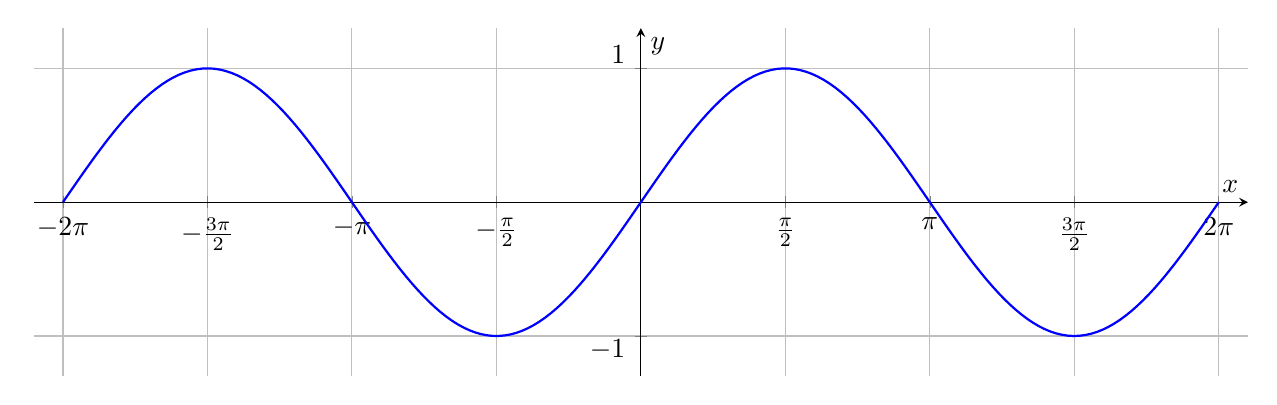
\begin{tikzpicture}
    \begin{axis}
        [
            width = 17cm,
            height = 6cm,
            axis lines = middle,
            xlabel = {$x$},
            ylabel = {$y$},
            xmin = -6.6,
            xmax = 6.6,
            ymin = -1.3,
            ymax = 1.3,
            xtick = {-6.2832, -4.7124, -3.1415, -1.5708, 0, 1.5708, 3.1415, 4.7124, 6.2832},
            xticklabels={
                    $-2\pi$,
                    $-\frac{3\pi}{2}$,
                    $-\pi$,
                    $-\frac{\pi}{2}$,
                    $0$,
                    $\frac{\pi}{2}$,
                    $\pi$,
                    $\frac{3\pi}{2}$,
                    $2\pi$
                },            
            ytick = {-1, 0, 1},
            yticklabel style = {yshift = {\tick*5pt}},
            grid = major, 
        ]

        \addplot
        [
            blue,
            thick,
            domain = -6.2832:6.2832,
            samples = 200
        ] {sin(deg(x))};
    \end{axis}
\end{tikzpicture}
